\chapter{Full Wave Rectification}
	\section{Aim}
		\begin{itemize}
			\tightlist
			\item Explain Rectification
			\item Explain Center Tapped Full Wave Rectification
			\item Explain Bridge Full Wave Rectification
		\end{itemize}
	
	\section{Apparatus}
		\begin{itemize}
			\tightlist
			\item Center Tapped Transformer
			\item Silicon Diodes
			\item AC Power Source
			\item Resistors
			\item Ammeter
			\item Voltmeter
		\end{itemize}
	
	\section{Theory}
		\subsection{Rectification}
			\begin{figure}[h]
				\centering
				
\includegraphics[width=0.9\linewidth]{img/exp7/1}
				\caption{Function of a Rectifier}
				\label{fig:rffwR}
			\end{figure}
			A rectifier is a device that converts alternating current (AC) to direct current (DC), a process known as rectification. Rectifiers are essentially of two types – a half wave rectifier and a full wave rectifier.
		
		\subsection{Full Wave Rectifier}
			A full-wave rectifier is exactly the same as the half-wave, but allows unidirectional current through the load during the entire sinusoidal cycle (as opposed to only half the cycle in the half-wave). A full-wave rectifier converts the whole of the input waveform to one of constant polarity (positive or negative) at its output. Let us see our half wave rectifier example and deduce the circuit.					
			For a half wave Rectifier this is what we have observed as in Figure \ref{fig:rfhw}. If we change the phase of the input waveform by 180 degrees, we get Figure \ref{fig:fwr_hwrBy180}. Now if we add these two circuits, we would get Figure \ref{fig:fwr_2hwrMerged}.
			\begin{figure}[ht]
				\centering 
				\subfloat[Full Wave Rectification]{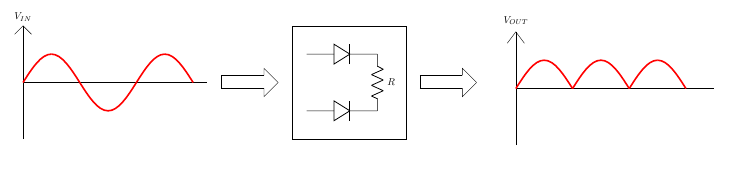
\includegraphics[width=0.9\textwidth]{img/exp7/2}
					\label{fig:fwrSinGraph}}
				\vfill
				\subfloat[Half Wave Rectification with Waveform changed by 180$^{\circ}$]{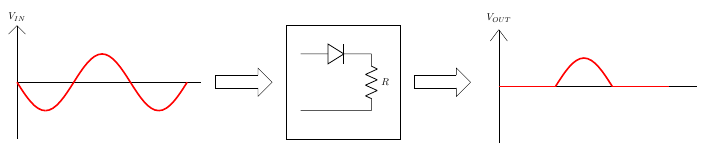
\includegraphics[width=0.9\textwidth,valign=c]{img/exp7/4}
					\label{fig:fwr_hwrBy180}}
				\vfill
				\subfloat[2 different Half Wave Rectifications]{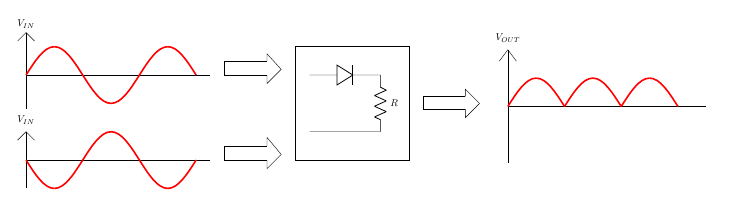
\includegraphics[width=0.9\textwidth,valign=c]{img/exp7/5}
					\label{fig:fwr_2hwrMerged}}
				\caption{\textit{How Full Wave Rectification can be obtained from Half-Wave Rectification}}
			\end{figure}
		
		\subsection{Full Wave Rectifier - Circuit}
			\begin{figure}[h]
				\centering
				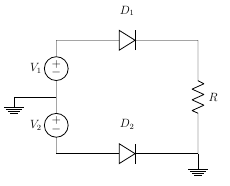
\includegraphics[width=0.5\linewidth]{img/exp7/6}
				\caption{Circuit of Full Wave Rectifier}
				\label{fig:fwr_fwrCircuit}
			\end{figure}
			So, we have seen that this rectifier circuit consists of two sources which have a phase difference along with two diodes(see Figure \ref{fig:fwr_fwrCircuit}) When $V_1$ is positive, $V_2$ is negative. Hence the top diode($D_1$) will be a short and the bottom diode($D_2$) will be an open.
			On the other hand, when $V_1$ is negative, $V_2$ is positive. Hence the bottom diode($D_2$) will be on and the top diode($D_1$) will be an open circuit.
			
		\subsection{Full Wave Rectifier – Waveforms}
			\begin{figure}[ht]
				\centering 
				\subfloat[Simple $sin x$ wave]{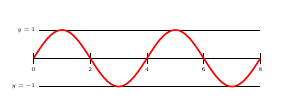
\includegraphics[width=0.45\textwidth, valign=c]{img/exp7/7}
					\label{fig:fwr_sin_waveform}}
				\subfloat[180$^{\circ}$ inverted $sin x$ wave]{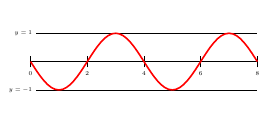
\includegraphics[width=0.45\textwidth,valign=c]{img/exp7/8}
					\label{fig:fwr_sin_180_waveform}}
				\vfill
				\subfloat[Rectified $\lvert sin x \rvert$ wave]{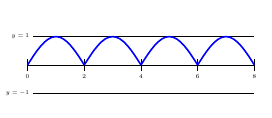
\includegraphics[width=0.9\textwidth,valign=c]{img/exp7/9}
					\label{fig:fwr_abs_sin_waveform}}
				\label{fig:fwr_waveform_wholeDiagram}
				\caption{\textit{Waveforms Resulting from Full Wave Rectifier}}
			\end{figure}
			The resulting waveform of the schematic is shown  in \ref{fig:fwr_sin_waveform}. This configuration is rarely used because sometimes it may be impractical to obtain two voltage sources and it is difficult to SYNC the sources. Let us see how a single source can be used.
		
		\subsection{Full Wave Rectifier – Center Tapped Transformer}
			A Full-Wave Rectifier can be constructed using Center-Tapped transformer (see Figure \ref{fig:fwr_centerTappedTransformer}) – which give us two shifted sinusoids so that exactly one of the waveforms is positive at one time and two diodes. As compared to the half wave rectifier we use two diodes instead of one, one of the two diodes remains in conduction in both of the half cycles. At any point in time, only one of the diodes is forward biased. This allows for continuous conduction through load.
			\begin{figure}[ht]
				\centering 
				\subfloat[Center-Tapped Transformer]{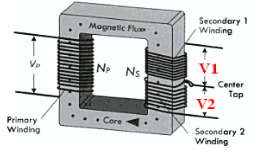
\includegraphics[width=0.4\textwidth]{img/exp7/10}
					\label{fig:fwr_centerTappedTransformer}}
				\hfill
				\subfloat[Symbol of Center-Tapped Transformer]{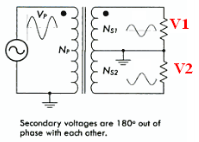
\includegraphics[width=0.4\textwidth,valign=c]{img/exp7/11}
					\label{fig:fwr_centerTappedTransformer_Symbol}}
				\caption{\textit{An AC Wave can be rectified with a center-tapped transformer}}
			\end{figure}
			$$\frac{N_P}{N_S}=\frac{V_P}{V_S}=\frac{1}{2}$$
			$$\Rightarrow V_S=2 \times V_I$$
			
			\subsubsection{Center Tapped Transformer – Positive cycle}
				\begin{figure}[h]
					\centering
					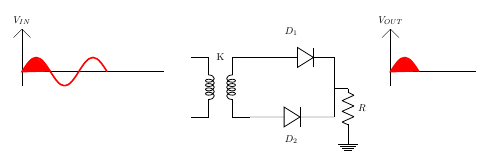
\includegraphics[width=0.9\linewidth]{img/exp7/12}
					\caption{Center Tapped Transformer – Positive cycle}
					\label{fig:fwr_centerTappedTranformer_positiveCycle}
				\end{figure}
				For Positive Cycle \(D_1\) is Forward Biased and \(D_2\) is Reverse Biased (See Figure \ref{fig:fwr_centerTappedTranformer_positiveCycle})
				$$V_I - V_O=0$$
				$$\Rightarrow V_O=V_I$$
				
			\subsubsection{Center Tapped Transformer– Negative cycle}
				\begin{figure}[h]
					\centering
					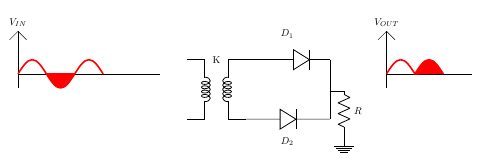
\includegraphics[width=0.9\linewidth]{img/exp7/13}
					\caption{Center Tapped Transformer – Negative cycle}
					\label{fig:fwr_centerTappedTranformer_negativeCycle}
				\end{figure}
				For Negative Cycle \(D_1\) is Reverse Biased and \(D_2\) is Forward Biased (See Figure \ref{fig:fwr_centerTappedTranformer_negativeCycle})
				$$V_I - V_O=0$$
				$$\Rightarrow V_O=V_I$$
		
		\subsection{Bridge Rectifier}
			\begin{figure}[h]
				\centering
				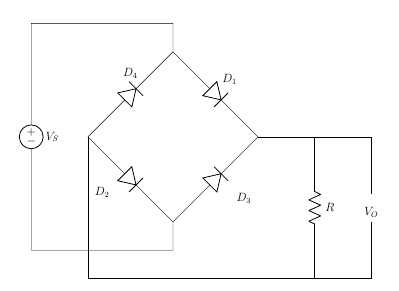
\includegraphics[width=0.5\linewidth]{img/exp7/14}
				\caption{A Bridge Rectifier}
				\label{fig:fwr_bridgeRectifier}
			\end{figure}
			Bridge rectifier uses 4 rectifying diodes connected in a "bridged" configuration(see Figure \ref{fig:fwr_bridgeRectifier}) to produce the desired output but does not require a special centre tapped transformer, thereby reducing its size and cost. The single secondary winding is connected to one side of the diode bridge network and the load to the other side as shown below.
			\begin{figure}[ht]
				\centering 
				\subfloat[Center-Tapped Transformer]{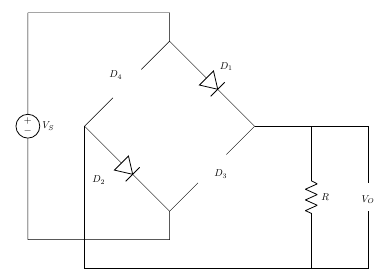
\includegraphics[width=0.45\textwidth]{img/exp7/15}
					\label{fig:fwr_bridgeRectifier_positiveCycle}}
				\hfill
				\subfloat[Symbol of Center-Tapped Transformer]{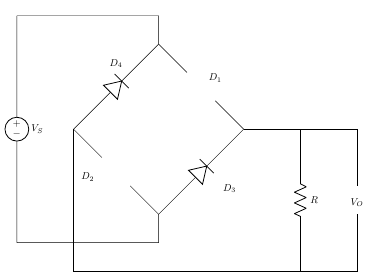
\includegraphics[width=0.45\textwidth,valign=c]{img/exp7/16}
					\label{fig:fwr_bridgeRectifier_negativeCycle}}
				\caption{\textit{Bridge Rectifier with positive and negative halves}}
			\end{figure}
			
			\subsubsection{Bridge Rectifier – Positive Half Cycle}
				During the positive half cycle of the supply diodes $D_1$ and $D_2$ conduct in series while diodes $D_3$ and $D_4$ are reverse biased (ideally they can be replaced with open circuits) and the current flows through the load as shown in Figure \ref{fig:fwr_bridgeRectifier_positiveCycle}.				
				For Positive Half Cycle \(D_1\) and \(D_2\) is Forward Biased and \(D_3\) and \(D_4\) is Reverse Biased. $$V_I-V_O=0$$
				$$\Rightarrow V_O=V_I$$
				$$V_O=V_I -2 \times V_b$$
				$$V_O=V_I -2 \times V_b - 2 \times I_{rd}$$
				where,
				\(V_I\) is the input voltage,
				\(V_b\) is barrier potential,
				\(r_d\) is diode resistance
				
			\subsubsection{Bridge Rectifier – Negative Half Cycle}
				During the negative half cycle of the supply, diodes $D_3$ and $D_4$ conduct in series, but diodes $D_1$ and $D_2$ switch of as they are now reverse biased. The current flowing through the load is the same direction as before. (see Figure \ref{fig:fwr_bridgeRectifier_negativeCycle})
				For Negative Half Cycle \(D_1\) and \(D_2\) is Reverse Biased and \(D_3\) and \(D_4\) is Forward Biased. $$V_I-V_O=0$$
				$$\Rightarrow V_O=V_I$$
		
		\subsection{Average DC Load Voltage}
			\begin{align*}
				V_O &= V_m \times \sin wt \quad for \quad 0 \leq wt \leq \pi\\
				V_{av} &= V_{dc}= \frac{2 \times V_m}{\pi}				
			\end{align*}
			
		\subsection{Average Load Current}
			\begin{align*}
				I_{av} &=\frac{V_{av}}{R}\\
				&= \frac{2\times V_m}{\pi \times R}\\
				&= \frac{2 \times I_m}{R}
			\end{align*}			
		
		\subsection{RMS Load Current}
			\begin{align*}		
				I &= I_m \times \sin wt \quad for \quad 0 \leq wt \leq \pi\\
				I_{rms} &= \frac{I_m }{\sqrt{2}}
			\end{align*}
		
		\subsection{RMS Load Voltage}
			\begin{align*}		
				V_{rms} &= I_{rms} \times R \\
				&= \frac{I_m}{\sqrt{2}} \times R\\
				&=\frac{V_m}{\sqrt{2}}
			\end{align*}
			
		\subsection{Form factor}
			It is defined as the ratio of rms load voltage and average load voltage.
			\begin{align*}
				FF &= \frac{V_{rms}}{V_{av}}\\
				&= \frac{\frac{V_{m}}{√2}}{\frac{2 \times V_m}{\pi}}\\
				&= \frac{\pi}{2√2}\\
				&= 1.11\\
				FF &\geq 1
			\end{align*}
		
		\subsection{Ripple Factor}
			\begin{align*}
				\gamma &= \sqrt{{FF}^2-1}\times 100\%\\
				&= \sqrt{{1.11}^2-1} \times 100\%\\
				&= 48.1\%
			\end{align*}
		
		\subsection{Efficiency}
			It is defined as ratio of DC power available at the load to the input AC power.
			\begin{align*}
				n\% &= \frac{P_{load}}{P_{in}} \times 100\%\\
				&= \frac {{I_{dc}^2} \times R}{{I_{rms}^2} \times R}\times 100\%\\
				&= \frac{\frac {4 \times I_{m}^2}{\pi^2}}{\frac{I_{m}^2}{2}}\times 100\%\\
				&= \frac{8}{\pi^2}\times 100\% \\
				&= 81.13\%
			\end{align*}
		
		\subsection{Peak Inverse Volatge}
			For rectifier applications, peak inverse voltage (PIV) or peak reverse voltage (PRV) is the maximum value of reverse voltage which occurs at the peak of the input cycle when the diode is reverse-biased.The portion of the sinusoidal waveform which repeats or duplicates itself is known as the cycle. The part of the cycle above the horizontal axis is called the positive half-cycle, the part of the cycle below the horizontal axis is called the negative half cycle. With reference to the amplitude of the cycle, the peak inverse voltage is specified as the maximum negative value of the sine-wave within a cycle's negative half cycle.
			
			For Bridge Rectifier,\\
			\(D_1\) and \(D_2\) is Forward Biased\\
			\(D_3\) and \(D_4\) is Reverse Biased\\
			$$ V_m-V_O=0$$
			$$\Rightarrow V_O=V_m$$
			$$- V_O+PIV=0$$
			$$\Rightarrow PIV=V_m$$
			$$PIV \geq V_m$$
			For Center Tapped Rectifier,\\
			\(D_2\) is Forward Biased,\\
			PIV at \(D_1\), $$ V_m-V_O=0$$
			$$\Rightarrow V_O=V_m$$
			$$V_O-PIV+V_m$$
			$$\Rightarrow PIV=2V_m$$
			$$PIV \geq 2V_m$$
		
	\section{Procedure}
		\begin{enumerate}
			\item Set the resistor \(R_L\).
			\item Click on 'ON' button to start the experiment.
			\item Click on 'Sine Wave' button to generate input waveform
			\item Click on 'Oscilloscope' button to get the rectified output.
			\begin{figure}[h]
				\centering
				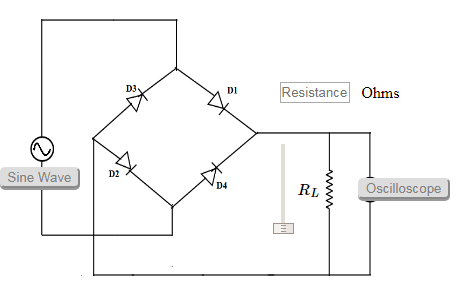
\includegraphics[width=0.5\linewidth]{img/exp7/17}
				\caption{Full Bridge Rectifier}
				\label{fig:fwr_procedure}
			\end{figure}
			\item Vary the Amplitude, Frequency, volt/div using the controllers.
			\item Click on "Dual" button to observe both the waveform.
			\item Channel 1 shows the input sine waveform, Channel 2 shows the output rectified waveform.
			\item Calculate the Ripple Factor.Theoretical Ripple Factor=0.483.
		\end{enumerate}
	
	\section{Calculation}
		 Measure the $V_m$
		 \begin{align*}
			V_{rms} &= \frac{V_m}{\sqrt{2}}\\	
			V_{dc} &= \frac{2 \times V_m} {\pi}\\
			Ripple Factor (RF) &=\frac{V_{ac}}{V_{dc}}\\
			Since, V_{ac} &=\sqrt{(V^2_{rms}-V^2_{dc})}
		 \end{align*}
	 	Peak Current: $0.599999 mA$
	 
	 \section{Observations}	
	 	\begin{figure}[h]
	 		\centering
	 		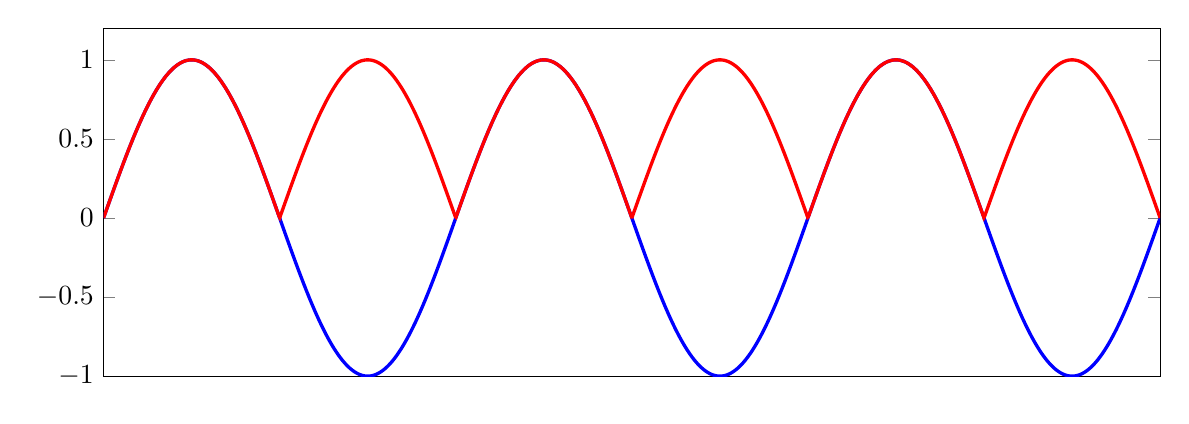
\begin{tikzpicture}
	 			\begin{axis}[
	 				domain=0:3*360,
	 				samples=4*360,
	 				xtick=\empty,
	 				width=15cm, height=6cm,
	 				ymin=-1,
	 				enlarge x limits=false
	 				]
	 				\addplot [blue, very thick] {sin(x)};
	 				\addplot [red, very thick] {abs(sin(x))};
	 			\end{axis}
	 		\end{tikzpicture}
	 		\caption{AC Wave Form (Blue), Full Wave Rectified Wave (Red)}
	 	\end{figure}	
 	
	 \section{Result}
	 	A full wave rectifier is defined as a type of rectifier that converts both halves of each cycle of an alternating wave (AC signal) into a pulsating DC signal. Full-wave rectifiers are used to convert AC voltage to DC voltage, requiring multiple diodes to construct. Full wave rectification is the process of converting an AC signal to a DC signal.
	 	
	 	Circuits that convert alternating current (AC) into direct current (DC) are known as rectifiers. If such rectifiers rectify both the positive and negative half cycles of an input alternating waveform, the rectifiers are full-wave rectifiers.
		
\afterpage{\clearpage}